\documentclass[a4paper]{article}

%use the english line for english reports
%usepackage[english]{babel}
\usepackage[portuguese]{babel}
\usepackage[utf8]{inputenc}
\usepackage{indentfirst}
\usepackage{graphicx}
\usepackage{verbatim}
\usepackage{listings}
\usepackage{booktabs}

\begin{document}

\setlength{\textwidth}{16cm}
\setlength{\textheight}{22cm}

\title{\Huge\textbf{Gestão de Elevadores}\linebreak\linebreak\linebreak
\Large\textbf{Relatório Final}\linebreak\linebreak
\linebreak\linebreak

\includegraphics[scale=0.1]{feup-logo.png}\linebreak\linebreak
\linebreak\linebreak
\Large{Mestrado Integrado em Engenharia Informática e Computação} \linebreak\linebreak
\Large{Agentes e Inteligência Artificial Distribuída}\linebreak
\Large{4º Ano 1º Semestre}\linebreak\linebreak
}

\author{\textbf{Grupo T01\_3:}\\ Luís  Barbosa - 201405729 - up201405729@fe.up.pt\\ Paulo Santos - 201403745 - up201403745@fe.up.pt \\ Sérgio Almeida  - 201403074 - up201403074@fe.up.pt \\\linebreak\linebreak \\
 \\ Faculdade de Engenharia da Universidade do Porto \\ Rua Roberto Frias, s/n, 4200-465 Porto, Portugal \linebreak\linebreak\linebreak
\linebreak\linebreak\vspace{1cm}}
\date{10 de dezembro de 2017}
\maketitle
\thispagestyle{empty}

%************************************************************************************************
%************************************************************************************************

\newpage

\tableofcontents

%************************************************************************************************
%************************************************************************************************

%*************************************************************************************************
%************************************************************************************************

\newpage

%%%%%%%%%%%%%%%%%%%%%%%%%%
\section{Objetivo}

\subsection{Descrição do cenário} 

O cenário do presente trabalho consiste num edifício de vários andares com diversos elevadores. Cada elevador possui uma carga máxima, que corresponde ao número máximo de pessoas que pode transportar.

Os elevadores comunicam entre si informação relevante. Quando há um novo pedido numa determinada zona do edifício, este deve ser alocado a um dos elevadores existentes naquela zona. Os elevadores possuem uma lista de pisos em que têm que parar, podendo a mesma ser alterada dinamicamente para se incluirem novos pedidos.

Periodicamente, os elevadores podem partilhar informação sobre os seus estados, no sentido de poderem atribuir tarefas a outros elevadores.

O programa deve permitir que o utilizador configure o sistema, como o número de pisos do edifício, número de elevadores e a carga máxima de cada elevador.

As necessidades dos utentes, como por exemplo a frequência de chamada de elevador em cada piso do edifício (devendo ser superior para o piso 0) e piso de destino, são geradas aleatoriamente. 

Um elevador demora um tempo pré-definido a ir de um piso a outro, sendo que o intervalo de tempo correspondente à paragem do elevador para entrada/saída de utentes também é contabilizado.

\subsection{Objetivos do trabalho} 

O trabalho tem como principal objetivo o desenvolvimento de um sistema multi-agente para a gestão eficiente dos elevadores de um determinado edifício, tendo em conta o cenário descrito acima. Para tal, será necessária a implementação de um algoritmo que permita gerir as chamadas aos elevadores de forma a que o transporte seja feito o mais rápido possível.

\newpage

%%%%%%%%%%%%%%%%%%%%%%%%%%
\section{Especificação}

\subsection{Identificação e caracterização dos agentes} 

No nosso projeto, distinguem-se dois tipos de agentes: \textit{Elevator} e \textit{Building}.

\subsubsection {\textit{Building}}

O \textit{Building} é instanciado apenas uma vez, assim que o programa é iniciado. Regista-se no \textit{DFService}, criando um \textit{DFAgentDescription}, adicionando a este um novo serviço com tipo "Building". Este agente é responsável por gerar elevadores e simular os pedidos existentes num edifício por parte dos utilizadores ao alocar aos elevadores os pedidos. Tem a seguinte \textbf{arquitetura}:

\begin{itemize}
\item \textbf{properties} - informações sobre o número de andares e elevadores, se existe teclado para efetuar pedido e se a negociação entre elevadores é permitida
\item \textbf{elevatorsProperties} - informações sobre o peso máximo, tempo de movimento e tempo de entrada/saída de pessoas
\item \textbf{elevators} - lista com o AID de todos os elevadores
\item \textbf{reqGenInterval} - valor do intervalo de geração de pedidos pelo edifício
\item \textbf{randNumRequestsPerInterval} - valor aleatório do número de pedidos gerados por intervalo, caso o valor lido do ficheiro seja "rand"
\item \textbf{numRequestsPerInterval} - valor lido do número de pedidos gerados por intervalo
\end{itemize}

Todas estas informações são lidas do ficheiro de configuração \textbf{default.properties}, de forma a tornar o processo de configuração do cenário mais generalizado.

Este agente tem o seguinte \textbf{comportamento}:

\begin{itemize}
\item Cria o número de pedidos definidos, definindo o andar inicial e, dependendo se existe teclado ou não, define um andar de destino diferente do inicial ou assume temporariamente que o andar de destino é o mesmo que o inicial. 
\item Cada pedido é atribuído ao elevador que indica um melhor tempo para levar o utilizador ao andar de destino, usando uma \textit{contract net}. 
\item Para isso, cria-se uma \textit{ACLMessage} do tipo \textit{CFP} com o seguinte conteúdo: \textbf{Andar Inicial, Andar Destino, Tempo para completar o pedido}. Esta é enviada pelo \textit{Building} para os \textbf{Elevator}, utilizando o protocolo de interação \textit{FIPA Contract Net}. Os \textbf{Elevator} irão retornar uma mensagem do tipo \textit{Propose} com o seu tempo até completar o pedido. O \textbf{Building} irá receber as respostas e escolher a melhor, enviando uma mensagem do tipo \textit{Accept Proposal} ao \textbf{Elevator} que enviou a melhor proposta. Por fim, o \textbf{Elevator} recetor irá enviar uma mensagem do tipo \textit{Inform} a indicar que recebeu a mensagem do tipo \textit{Accept Proposal}\end{itemize}

\subsubsection {\textit{Elevator}}

O \textit{Elevator} regista-se no serviço do \textit{Directory Facilitator} com o tipo "Elevator", de forma a que o \textit{Building} (e outros que subscrevam o \textit{Directory Facilitator}) saiba que este existe. Tem a seguinte \textbf{arquitetura}:

\begin{itemize}
\item \textbf{properties} -  informações sobre o peso máximo, tempo de movimento, tempo de entrada/saída de pessoas
\item \textbf{state} - informações sobre o piso atual, peso atual, estado de movimento ("STOPPED", "GOING\_UP" ou "GOING\_DOWN") e nº de pessoas
\item \textbf{internalRequests} - lista interna de pedidos a realizar, que é dinâmica, uma vez que pode ser alterada caso outros elevadores lhe atribuam um novo pedido, ou caso seja feito um novo pedido no \textit{Building}
\item \textbf{statistics} - estatísticas utilizadas na interface
\item \textbf{startupTime} – momento em que foi iniciado
\end{itemize}

Este agente tem o seguinte \textbf{comportamento}:

Caso a negociação entre elevadores seja permitida, tenta negociar com outros elevadores os pedidos internos, através do envio de uma \textit{ACLMessage} do tipo \textit{CFP}, utilizando o protocolo de interação \textit{FIPA Contract Net}. Os outros elevadores são adicionados como recetores da mensagem, usando o Directory Facilitator. Para cada pedido que ainda não tenha sido atendido, é procurado o pedido que vai ser mais demorado a executar, sendo esse pedido enviado pelo \textit{Elevator} que gera um \textit{Contract Net Initiator Behaviour}.

É feita a verificação da existência de algum pedido para o piso atual do elevador, e se ainda não foi atendido. Caso isto se verifique, o elevador para e é gerado um novo peso que não exceda a capacidade do mesmo. Este peso pretende simular a entrada de uma pessoa. Existem casos em que é gerado o valor 0 de forma a aproximar a uma situação real, pois por vezes não é possível satisfazer o pedido pois o elevador já se encontra lotado. Durante o tempo de entrada de pessoas, só são atendidos pedidos com piso inicial nesse andar.

A forma de o elevador decidir para que andar se deve dirigir tem por base o andar mais próximo do atual. É verificado todo o conjunto de pedidos do elevador, isto é, caso já tenha sido um pedido atendido, verifica-se qual é o andar de destino mais próximo. Caso seja um pedido externi, verifica-se qual é o andar de partida mais próximo.

O algoritmo de decisão tenta, em todos os andares, otimizar a distância ao próximo andar. Desta forma, garantimos que não ande um grande número de andares sem parar quando era mais eficiente ter parado a meio para atender mais pedidos.

Verifica, também, para todos os pedidos atendidos do elevador, se estes já se encontram no andar de destino. Quanto isto acontece, o elevador para e é simulada a saída da pessoa que tinha feito o pedido.

\subsection{Estratégias e processos de raciocínio} 

De forma a comparar o desempenho dos elevadores com diferentes heurísticas, foram implementadas quatro estratégias de alocação de pedidos. Estas quatro estratégias suportam um dos seguintes modelos: o primeiro, em que existe apenas um botão de chamada, ou um segundo que assume a existência de um teclado onde é possível indicar o piso de destino.

A \textbf{primeira} estratégia assume o sistema tradicional onde cada elevador possui uma estratégia fixa e individual e segue o primeiro modelo: atende o pedido o elevador que se encontra mais próximo do piso onde a chamada foi efetuada. Para isto ser possível, os elevadores comunicam entre si através do protocolo de interação que será descrito mais à frente. 

Para tornar o envio de requests para outros elevadores melhor, seria necessário pedir-lhes feedback para todos os requests e isso sobrecarregaria a rede de negociação, só se pedindo ajuda para o pior pedido de cada vez. Se não podem ajudar para o pior, provavelmente não podem ajudar para outros. E iterativamente, ao alocar os piores pedidos a outros, optimiza-se/reduz-se os tempos de espera.

A \textbf{segunda} estratégia segue o segundo modelo, onde o elevador já possui a informação de qual é o piso de destino, conseguindo calcular o tempo de espera exato, permitindo uma alocação mais correta dos pedidos.

As duas estratégias anteriores utilizam o protocolo de interação descrito abaixo para que os elevadores negoceiem entre si. Para termos melhores termos de comparação, achamos correto criar outras duas estratégias em que não existe negociação.

Desta forma, a \textbf{terceira} estratégia é idêntica à primeira e a \textbf{quarta} idêntica à segunda, exceto na parte em que negoceiam. Assim, ambas estimam o tempo que o elevador demoraria a responder a um pedido caso fosse alocado a ele.

\subsection{Protocolos de interação} 

O protocolo de interação utilizado na decisão para alocação de pedidos aos elevadores é o \textbf{FIPA CONTRACT NET}.

A cada período de geração de pedidos do \textit{Building} (reqGenInterval), para cada um destes é gerada uma \textit{ACLMessage} do tipo \textit{CFP}, com o protocolo \textbf{FIPA\_CONTRACT\_NET}, em que os os seus recetores são todos os elevadores do edifício. Em seguida, cada elevador após receber o \textbf{CFP}, calcula o tempo que vai demorar até ao andar inicial do pedido. Se este for menor do que o tempo que vem no pedido, o elevador envia uma \textit{ACLMessage} do tipo \textbf{PROPOSE}. Caso contrário, o agente envia uma \textit{ACLMessage} do tipo \textbf{REFUSE}. Quando o edifício recebe as propostas (\textit{ACLMessage} do tipo \textbf{PROPOSE}), analisa a melhor com base nos tempos e envia uma \textit{ACLMessage} do tipo \textbf{REJECT\_PROPOSAL} para todas, exceto para a melhor proposta, em que envia uma \textit{ACLMessage} do tipo \textbf{ACCEPT\_PROPOSAL}, ficando assim alocado o pedido a este elevador.

Também um elevador pode negociar o seu pior pedido com os restantes elevadores: assim, cria uma mensagem do tipo \textbf{CFP} com a informação do seu pior pedido e envia para os restantes elevadores. A gestão da receção deste pedido é feita de forma igual à da receção de pedidos do \textit{Building}. Caso não consiga atribuir a outro elevador, o pedido mantém-se alocado ao próprio. 

\begin{center}
	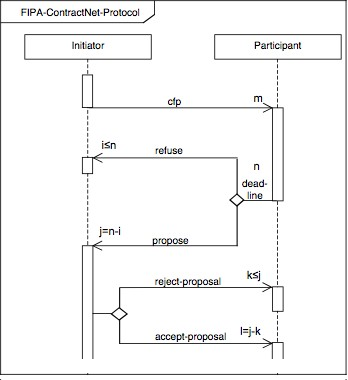
\includegraphics[scale=0.59]{fipa.png}
\end{center}

\newpage

%%%%%%%%%%%%%%%%%%%%%%%%%%
\section{Desenvolvimento}

\subsection{Plataforma/ferramenta utilizada e ambiente de desenvolvimento} 

A ferramenta escolhida para o desenvolvimento deste trabalho foi JADE. JADE é uma framework que permite o desenvolvimento de sistemas multiagente e é compatível com FIPA, isto é, segue os padrões de software estabelecidos para agentes heterogéneos e interativos e para sistemas baseados em agentes.

O projeto foi desenvolvido utilizando o IntelliJ IDEA Community Edition no sistema operativo Windows 10.

\subsection{Estrutura da aplicação} 

\begin{center}
\hspace*{-3.2cm}
	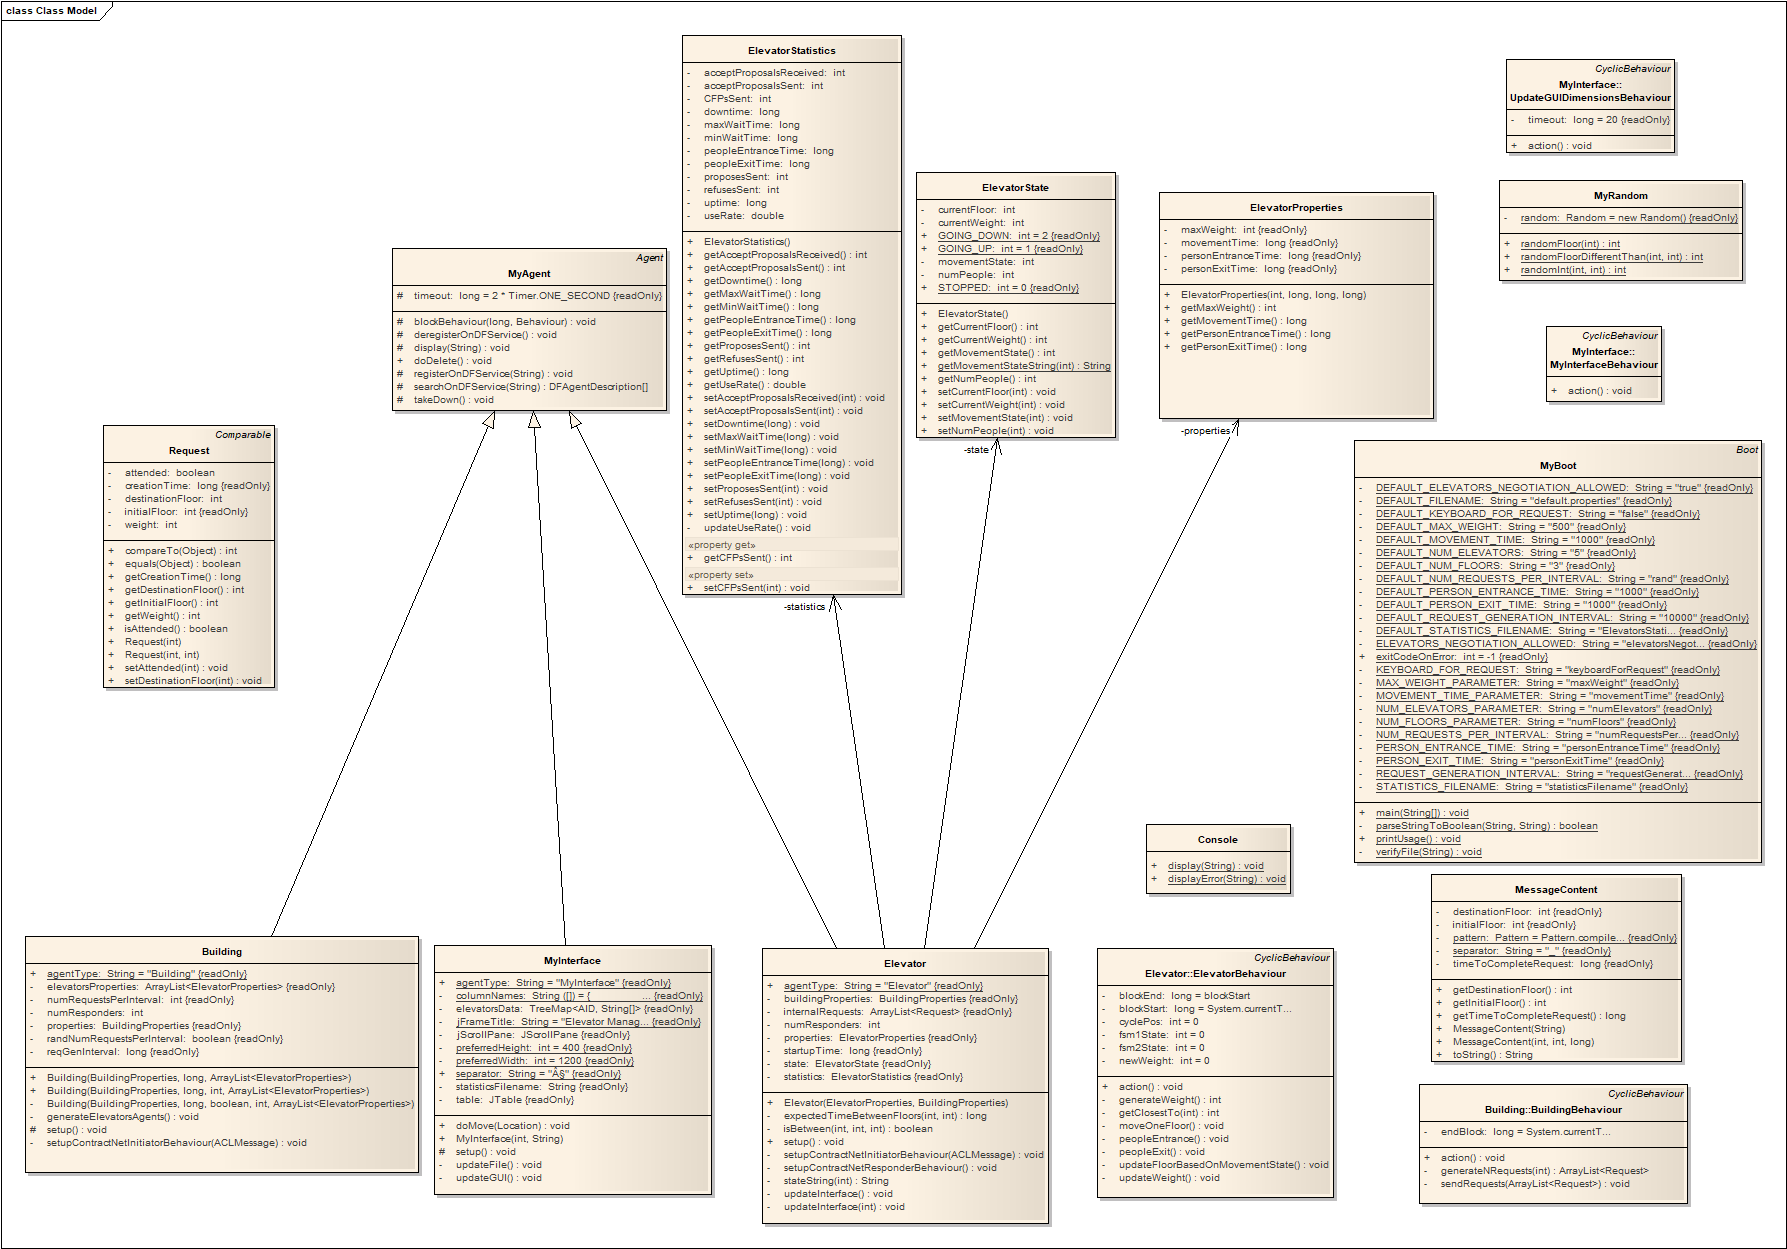
\includegraphics[scale=0.3]{class_model.png}\linebreak\linebreak
\end{center}

\subsection{Detalhes relevantes da implementação} 

Todo o projeto foi desenvolvido de forma a minimizar a possibilidade de ocorrerem erros, sendo que a classe mais complexa é a classe 'Elevator' que implementa uma máquina de estados complexa no seu "ElevatorBehaviour". Todos os outros agentes também implementam uma máquina de estados nos seus "Behaviour", mas são máquinas de estados muito simples.

A classe 'MyBoot' é a classe por onde o programa arranca, sendo que esta vai ler os parâmetros definidos na consola ou num ficheiro e inicia um agente do tipo 'Building' e outro do tipo 'MyInterface'.

A classe 'Building' por sua vez vai iniciar um conjunto de agentes do tipo 'Elevator'.

Todos os agentes criados são descendentes da classe 'MyAgent' que extende 'Agent' e implementa alguns métodos tranversais aos nossos diversos agentes.

O 'Building' tem um intervalo de tempo definido pelo utilizador para gerar novos pedidos, sendo que, de cada vez, gera um conjunto de pedidos e inicia uma \textit{contract net} para alocar cada pedido ao melhor elevador.

Já os elevadores escolhem da sua lista de pedidos aquele que apresenta o maior tempo entre quando foi criado e quando estará completamente atendido, ou seja, a pessoa estará no andar de destino desejado. Com este pedido, iniciam uma \textit{contract net} e alocam o pedido ao elevador que levar menos tempo a levar a pessoa até ao seu piso de destino (este cálculo inclui o tempo até chegar ao piso do pedido mais o tempo previsto até chegar ao destino). É iniciada, por cada elevador, uma \textit{contract net} com um pedido a cada 2 segundos. Por cada andar que o elevador anda, vê se deve deixar sair pessoas, vê se há pessoas a entrar, reavalia qual o melhor piso como próximo destino (escolhe o destino ou piso inicial mais próximo, sendo que para escolher um piso inicial tem de ser possível a entrada de mais pessoas) e move um andar se houver algum pedido para outro piso.

Para escolher os recetores das mensagens, tanto o 'Building' como os 'Elevator' usam o DirectoryFacilitator para encontrar os elevadores e assim adicioná-los como recetores. Eles são pesquisados com base no seu tipo e, se for um elevador a enviar, ele não envia a si mesmo.

A classe 'MyInterface' é um agente que não deve ser movido para outra máquina que cria uma interface gráfica e um ficheiro, apresentando dados sobre a situação atual de cada elevador e guardando esses dados num ficheiro definido pelo utilizador. A interface gráfica e o ficheiro são atualizados sempre que é recebida uma mensagem dirigida ao agente 'MyInterface' contendo os novos dados de um elevador.

Existe um conjunto de classes que serve para guardar informação de forma organizada, algumas que disponibilizam funções bastantes utilizadas em todo o programa e a classe 'MessageContent' a transformação da informação necessária à \textit{contract net} de variáveis para string e, ao contrário, de string a variáveis.

\newpage

%%%%%%%%%%%%%%%%%%%%%%%%%%
\section{Experiências}

De seguida, serão detalhadas algumas das experiências efetuadas de forma a ser possível tirar conclusões dos resultados, analisando as estratégias implementadas e a sua adaptação à variação das condições. De notar que para a realização destas experiências, o tempo de movimentação dos elevadores e a capacidade máxima é igual para todos os elevadores. No entanto, o nosso programa permite que os valores sejam diferentes. Pensamos que o mais correto para conseguirmos concluir algo sobre as estratégias era que todos os elevadores tivessem as mesmas condições entre eles, fazendo-as variar (de igual forma entre eles) de experiência para experiência, pois caso contrário iriam existir elevadores a comportarem-se de uma melhor forma entre eles e não implicaria que fosse devido à estratégia.

Todos os resultados foram recolhidos após 2 minutos a correr o programa.

\subsection{Experiência 1}

\subsubsection{Condições iniciais}

\begin{itemize}
\item \textbf{numFloors}=10
\item \textbf{numElevators}=3
\item \textbf{requestGenerationInterval}=10000(ms)
\item \textbf{numRequestsPerInterval}=2
\item \textbf{maxWeigt Elevator 0,1,2}=[500, 500, 500]
\item \textbf{movementTime Elevator 0, 1, 2}=[1000, 1000, 1000]
\end{itemize}

\subsubsection{Objetivo} 

O objetivo desta experiência consiste em comparar os resultados das várias estratégias implementadas com as mesmas condições para todos os elevadores.

\subsubsection{Resultados}

Utilizando a primeira estratégia,

\begin{table}[h]
\centering
\hspace*{-3.2cm}
\begin{tabular}{@{}llllllllll@{}}
\toprule
Agent     & \begin{tabular}[c]{@{}l@{}}CFPs\\ sent \end{tabular} & \begin{tabular}[c]{@{}l@{}}Proposes\\ sent\end{tabular} & \begin{tabular}[c]{@{}l@{}}Refuses\\ sent\end{tabular} & \begin{tabular}[c]{@{}l@{}}Accept\\ proposals sent\end{tabular} & \begin{tabular}[c]{@{}l@{}}Accept proposals\\ received\end{tabular} & \begin{tabular}[c]{@{}l@{}}Max wait\\ time (ms)\end{tabular} & \begin{tabular}[c]{@{}l@{}}Uptime\\ (ms)\end{tabular} & \begin{tabular}[c]{@{}l@{}}Downtime\\ (ms)\end{tabular} &\begin{tabular}[c]{@{}l@{}}Use \\rate (\%) \end{tabular} \\ \midrule
Elevator0 & 14        & 28            & 18           & 2                                                               & 11                                                                  & 7048                                                         & 53118                                                 & 61237                                                   & 46.45         \\
Elevator1 & 13        & 30            &  17           & 3                                                               & 15                                                                  & 6017                                                         & 47065                                                 & 73290                                                   & 39.105         \\
Elevator2 & 8        & 29            & 23           & 4                                                               & 8                                                                  & 2009                                                         & 59955                                                 & 59397                                                   & 50.23         \\
Average   & 11.66     & 29         & 19.3        & 3                                                              & 11.3                                                            & 5025                                                         & 53379                                                 & 64641                                                   & 45.26         \\ \bottomrule
\end{tabular}
\end{table}

\newpage

Utilizando a segunda estratégia,

\begin{table}[h]
\centering
\hspace*{-3.2cm}
\begin{tabular}{@{}llllllllll@{}}
\toprule
Agent     & \begin{tabular}[c]{@{}l@{}}CFPs\\ sent \end{tabular} & \begin{tabular}[c]{@{}l@{}}Proposes\\ sent\end{tabular} & \begin{tabular}[c]{@{}l@{}}Refuses\\ sent\end{tabular} & \begin{tabular}[c]{@{}l@{}}Accept\\ proposals sent\end{tabular} & \begin{tabular}[c]{@{}l@{}}Accept proposals\\ received\end{tabular} & \begin{tabular}[c]{@{}l@{}}Max wait\\ time (ms)\end{tabular} & \begin{tabular}[c]{@{}l@{}}Uptime\\ (ms)\end{tabular} & \begin{tabular}[c]{@{}l@{}}Downtime\\ (ms)\end{tabular} &\begin{tabular}[c]{@{}l@{}}Use \\rate (\%) \end{tabular} \\ \midrule
Elevator0 & 7        & 30            & 11           & 2                                                               & 10                                                                  & 3005 & 40101                                                 & 66248                                                   & 37.71         \\
Elevator1 &  9       & 25            & 14           & 2                                                               & 11                                                                  & 4007                                                         & 48087                                                 & 73301                                                   & 39.61         \\
Elevator2 & 7        & 27            & 14           & 3                                                               & 11                                                                  & 3007                                                         & 27037                                                 & 65307                                                   & 29.28         \\
Average   & 7.66     & 27.33         & 13        & 2.33                                                               & 10.67 & 3340                                                         & 38408                                                 & 68285                                                   & 35.71          \\ \bottomrule
\end{tabular}
\end{table}

Utilizando a terceira estratégia,

\begin{table}[h]
\centering
\hspace*{-3.2cm}
\begin{tabular}{@{}llllllllll@{}}
\toprule
Agent     & \begin{tabular}[c]{@{}l@{}}CFPs\\ sent \end{tabular} & \begin{tabular}[c]{@{}l@{}}Proposes\\ sent\end{tabular} & \begin{tabular}[c]{@{}l@{}}Refuses\\ sent\end{tabular} & \begin{tabular}[c]{@{}l@{}}Accept\\ proposals sent\end{tabular} & \begin{tabular}[c]{@{}l@{}}Accept proposals\\ received\end{tabular} & \begin{tabular}[c]{@{}l@{}}Max wait\\ time (ms)\end{tabular} & \begin{tabular}[c]{@{}l@{}}Uptime\\ (ms)\end{tabular} & \begin{tabular}[c]{@{}l@{}}Downtime\\ (ms)\end{tabular} &\begin{tabular}[c]{@{}l@{}}Use \\rate (\%) \end{tabular} \\ \midrule
Elevator0 & 0        & 25            & 0           & 0                                                               & 4                                                                  & 3009                                                         & 24037                                                 & 94616                                                   & 20.26         \\
Elevator1 & 0        & 26           & 0           & 0                                                               & 10                                                                  & 6016                                                         & 42110                                                 & 64551                                                   & 39.48         \\
Elevator2 & 0        & 25            & 0           & 0                                                               & 10                                                                  & 5001                                                         & 43072                                                 & 77594                                                   & 35.7         \\
Average   & 0     & 25.33         & 0        & 0                                                               & 8                                                               & 4675                                                         & 36406                                                 & 78920                                                   & 31.81          \\ \bottomrule
\end{tabular}
\end{table}

Utilizando a quarta estratégia,

\begin{table}[h]
\centering
\hspace*{-3.2cm}
\begin{tabular}{@{}llllllllll@{}}
\toprule
Agent     & \begin{tabular}[c]{@{}l@{}}CFPs\\ sent \end{tabular} & \begin{tabular}[c]{@{}l@{}}Proposes\\ sent\end{tabular} & \begin{tabular}[c]{@{}l@{}}Refuses\\ sent\end{tabular} & \begin{tabular}[c]{@{}l@{}}Accept\\ proposals sent\end{tabular} & \begin{tabular}[c]{@{}l@{}}Accept proposals\\ received\end{tabular} & \begin{tabular}[c]{@{}l@{}}Max wait\\ time (ms)\end{tabular} & \begin{tabular}[c]{@{}l@{}}Uptime\\ (ms)\end{tabular} & \begin{tabular}[c]{@{}l@{}}Downtime\\ (ms)\end{tabular} &\begin{tabular}[c]{@{}l@{}}Use \\rate (\%) \end{tabular} \\ \midrule
Elevator0 & 0        & 24            & 0           & 0                                                               & 6                                                                  & 4015                                                         & 30044                                                 & 84393                                                   & 26.25         \\
Elevator1 & 0        & 25           & 0           & 0                                                               & 11                                                                  & 17447                                                         & 80198                                                 & 38258                                                   & 67.7         \\
Elevator2 & 0        & 25            & 0           & 0                                                               & 7                                                                  & 8019                                                         & 47104                                                 & 56341                                                   & 45.54         \\
Average   & 0     & 24.67         & 0        & 0                                                               & 8                                                               & 9827                                                         & 52449                                                 &  59664                                                  & 46.5          \\ \bottomrule
\end{tabular}
\end{table}

\subsection{Experiência 2}

\subsubsection{Condições iniciais}

\begin{itemize}
\item \textbf{numFloors}=10
\item \textbf{numElevators}=3
\item \textbf{requestGenerationInterval}=10000(ms)
\item \textbf{numRequestsPerInterval}=2
\item \textbf{maxWeigt Elevator 0,1,2}=[500, 500, 500]
\item \textbf{movementTime Elevator 0, 1, 2}=[300, 300, 300]
\end{itemize}

\subsubsection{Objetivo} 

O objetivo desta experiência consiste em comparar os resultados das várias estratégias implementadas com as mesmas condições para todos os elevadores, mas com velocidade mais rápida comparada com a experiência anterior.

\newpage
\subsubsection{Resultados}

Utilizando a primeira estratégia,

\begin{table}[h]
\centering
\hspace*{-3.2cm}
\begin{tabular}{@{}llllllllll@{}}
\toprule
Agent     & \begin{tabular}[c]{@{}l@{}}CFPs\\ sent \end{tabular} & \begin{tabular}[c]{@{}l@{}}Proposes\\ sent\end{tabular} & \begin{tabular}[c]{@{}l@{}}Refuses\\ sent\end{tabular} & \begin{tabular}[c]{@{}l@{}}Accept\\ proposals sent\end{tabular} & \begin{tabular}[c]{@{}l@{}}Accept proposals\\ received\end{tabular} & \begin{tabular}[c]{@{}l@{}}Max wait\\ time (ms)\end{tabular} & \begin{tabular}[c]{@{}l@{}}Uptime\\ (ms)\end{tabular} & \begin{tabular}[c]{@{}l@{}}Downtime\\ (ms)\end{tabular} &\begin{tabular}[c]{@{}l@{}}Use \\rate (\%) \end{tabular} \\ \midrule
Elevator0 & 4        & 27            & 12           & 3                                                               & 8                                                                  & 1902                                                         & 13682                                                 & 101232                                                   & 11.91         \\
Elevator1 & 8        & 28            & 7           & 2                                                               & 14                                                                  & 3512                                                         & 21973                                                 & 98716                                                   & 18.2        \\
Elevator2 & 6        & 26            & 12           & 0                                                               & 9                                                                  & 4135                                                         & 12792                                                 & 107895                                                   & 10.59         \\
Average   & 6     & 27         & 10.33        & 1.67                                                               & 10.33                                                               & 3183                                                         & 16149                                                 & 102614                                                   & 10.56          \\ \bottomrule
\end{tabular}
\end{table}

Utilizando a segunda estratégia,

\begin{table}[h]
\centering
\hspace*{-3.2cm}
\begin{tabular}{@{}llllllllll@{}}
\toprule
Agent     & \begin{tabular}[c]{@{}l@{}}CFPs\\ sent \end{tabular} & \begin{tabular}[c]{@{}l@{}}Proposes\\ sent\end{tabular} & \begin{tabular}[c]{@{}l@{}}Refuses\\ sent\end{tabular} & \begin{tabular}[c]{@{}l@{}}Accept\\ proposals sent\end{tabular} & \begin{tabular}[c]{@{}l@{}}Accept proposals\\ received\end{tabular} & \begin{tabular}[c]{@{}l@{}}Max wait\\ time (ms)\end{tabular} & \begin{tabular}[c]{@{}l@{}}Uptime\\ (ms)\end{tabular} & \begin{tabular}[c]{@{}l@{}}Downtime\\ (ms)\end{tabular} &\begin{tabular}[c]{@{}l@{}}Use \\rate (\%) \end{tabular} \\ \midrule
Elevator0 & 5        & 26            & 4           & 1                                                               & 12                                                                  & 2205                                                         & 19637                                                 & 93603                                                   & 17.34         \\
Elevator1 & 3        & 25            & 7           & 0                                                               & 8                                                                  & 1914                                                         & 13969                                                 & 107055                                                   & 11.54         \\
Elevator2 & 1        & 26            & 6           & 0                                                               & 7                                                                  & 2204                                                         & 10850                                                 & 102684                                                   & 9.56         \\
Average   & 3     & 25.67         & 5.67        & 0.33                                                               & 9                                                               & 2108                                                         & 14819                                                 & 101114                                                   &  12.81         \\ \bottomrule
\end{tabular}
\end{table}

Utilizando a terceira estratégia,

\begin{table}[h]
\centering
\hspace*{-3.2cm}
\begin{tabular}{@{}llllllllll@{}}
\toprule
Agent     & \begin{tabular}[c]{@{}l@{}}CFPs\\ sent \end{tabular} & \begin{tabular}[c]{@{}l@{}}Proposes\\ sent\end{tabular} & \begin{tabular}[c]{@{}l@{}}Refuses\\ sent\end{tabular} & \begin{tabular}[c]{@{}l@{}}Accept\\ proposals sent\end{tabular} & \begin{tabular}[c]{@{}l@{}}Accept proposals\\ received\end{tabular} & \begin{tabular}[c]{@{}l@{}}Max wait\\ time (ms)\end{tabular} & \begin{tabular}[c]{@{}l@{}}Uptime\\ (ms)\end{tabular} & \begin{tabular}[c]{@{}l@{}}Downtime\\ (ms)\end{tabular} &\begin{tabular}[c]{@{}l@{}}Use \\rate (\%) \end{tabular} \\ \midrule
Elevator0 & 0        & 25            & 0           & 0                                                               & 7                                                                  & 905                                                         & 13654                                                 & 91214                                                   & 13.02         \\
Elevator1 & 0        & 24           & 0           & 0                                                               & 9                                                                  & 2431                                                         & 15760                                                 & 79995                                                   & 16.46         \\
Elevator2 & 0        & 25            & 0           & 0                                                               & 8                                                                  & 5330                                                         & 12994                                                 & 103176                                                   & 11.19         \\
Average   & 0     & 24.67         & 0        & 0                                                               & 8                                                              & 2889                                                         & 14136                                                 &  91462                                                  & 13.55         \\ \bottomrule
\end{tabular}
\end{table}

\newpage

Utilizando a quarta estratégia,

\begin{table}[h]
\centering
\hspace*{-3.2cm}
\begin{tabular}{@{}llllllllll@{}}
\toprule
Agent     & \begin{tabular}[c]{@{}l@{}}CFPs\\ sent \end{tabular} & \begin{tabular}[c]{@{}l@{}}Proposes\\ sent\end{tabular} & \begin{tabular}[c]{@{}l@{}}Refuses\\ sent\end{tabular} & \begin{tabular}[c]{@{}l@{}}Accept\\ proposals sent\end{tabular} & \begin{tabular}[c]{@{}l@{}}Accept proposals\\ received\end{tabular} & \begin{tabular}[c]{@{}l@{}}Max wait\\ time (ms)\end{tabular} & \begin{tabular}[c]{@{}l@{}}Uptime\\ (ms)\end{tabular} & \begin{tabular}[c]{@{}l@{}}Downtime\\ (ms)\end{tabular} &\begin{tabular}[c]{@{}l@{}}Use \\rate (\%) \end{tabular} \\ \midrule
Elevator0 & 0        & 26            & 0           & 0                                                               & 10                                                                  & 3810                                                         & 19064                                                 & 88452                                                   & 17.73         \\
Elevator1 & 0        & 26           & 0           & 0                                                               & 4                                                                  & 4                                                         & 5734                                                 & 115889                                                   & 4.71         \\
Elevator2 & 0        & 25            & 0           & 0                                                               & 12                                                                  & 3810                                                         & 23214                                                 & 91719                                                   & 20.2         \\
Average   & 0     & 25.67         & 0        & 0                                                               & 8.67                                                              & 2541                                                         & 16004                                                 &  96687                                                  & 14.21        \\ \bottomrule
\end{tabular}
\end{table}

\subsection{Experiência 3}

\subsubsection{Condições iniciais}

\begin{itemize}
\item \textbf{numFloors}=5
\item \textbf{numElevators}=3
\item \textbf{requestGenerationInterval}=10000(ms)
\item \textbf{numRequestsPerInterval}=2
\item \textbf{maxWeigt Elevator 0,1,2}=[500, 500, 500]
\item \textbf{movementTime Elevator 0, 1, 2}=[1000, 1000, 1000]
\end{itemize}

\subsubsection{Objetivo} 

O objetivo desta experiência consiste em comparar os resultados das várias estratégias implementadas com as mesmas condições para todos os elevadores, mas com um número de pisos inferior.

\subsubsection{Resultados}

Utilizando a primeira estratégia,

\begin{table}[h]
\centering
\hspace*{-3.2cm}
\begin{tabular}{@{}llllllllll@{}}
\toprule
Agent     & \begin{tabular}[c]{@{}l@{}}CFPs\\ sent \end{tabular} & \begin{tabular}[c]{@{}l@{}}Proposes\\ sent\end{tabular} & \begin{tabular}[c]{@{}l@{}}Refuses\\ sent\end{tabular} & \begin{tabular}[c]{@{}l@{}}Accept\\ proposals sent\end{tabular} & \begin{tabular}[c]{@{}l@{}}Accept proposals\\ received\end{tabular} & \begin{tabular}[c]{@{}l@{}}Max wait\\ time (ms)\end{tabular} & \begin{tabular}[c]{@{}l@{}}Uptime\\ (ms)\end{tabular} & \begin{tabular}[c]{@{}l@{}}Downtime\\ (ms)\end{tabular} &\begin{tabular}[c]{@{}l@{}}Use \\rate (\%) \end{tabular} \\ \midrule
Elevator0 & 5        & 33            & 13           & 16                                                               & 2                                                                  & 2002                                                         & 39053                                                 & 82615                                                   & 33.1         \\
Elevator1 & 17        & 29            & 20           & 8                                                               & 6                                                                  & 4003                                                         & 40152                                                 & 81255                                                   & 33.1        \\
Elevator2 & 6        & 29            & 10           & 19                                                               & 2                                                                  & 4336                                                         & 30368                                                 & 49317                                                   & 38.1         \\
Average   & 9.33     & 30.33         & 14.33        & 14.33                                                               & 3.33                                                               & 3447                                                         & 36524                                                 & 71062                                                   & 34.8          \\ \bottomrule
\end{tabular}
\end{table}

Utilizando a segunda estratégia,

\begin{table}[h]
\centering
\hspace*{-3.2cm}
\begin{tabular}{@{}llllllllll@{}}
\toprule
Agent     & \begin{tabular}[c]{@{}l@{}}CFPs\\ sent \end{tabular} & \begin{tabular}[c]{@{}l@{}}Proposes\\ sent\end{tabular} & \begin{tabular}[c]{@{}l@{}}Refuses\\ sent\end{tabular} & \begin{tabular}[c]{@{}l@{}}Accept\\ proposals sent\end{tabular} & \begin{tabular}[c]{@{}l@{}}Accept proposals\\ received\end{tabular} & \begin{tabular}[c]{@{}l@{}}Max wait\\ time (ms)\end{tabular} & \begin{tabular}[c]{@{}l@{}}Uptime\\ (ms)\end{tabular} & \begin{tabular}[c]{@{}l@{}}Downtime\\ (ms)\end{tabular} &\begin{tabular}[c]{@{}l@{}}Use \\rate (\%) \end{tabular} \\ \midrule
Elevator0 & 7        & 25            & 12           & 2                                                               & 12                                                                  & 2088                                                         & 33146                                                 & 79417                                                   & 29.45        \\
Elevator1 & 6        & 27            & 11           & 2                                                               & 9                                                                  & 1052                                                         & 19053                                                 & 57371                                                   & 24.93         \\
Elevator2 & 7        & 27            & 10           & 1                                                               & 8                                                                  & 5005                                                         & 22029                                                 & 91533                                                   & 19.4         \\
Average   & 6.67     & 26.33         & 11        & 1.67                                                            & 9.33                                                               & 1936.67                                                         & 24743                                                 & 76107                                                   &  24.6         \\ \bottomrule
\end{tabular}
\end{table}

\newpage

Utilizando a terceira estratégia,

\begin{table}[h]
\centering
\hspace*{-3.2cm}
\begin{tabular}{@{}llllllllll@{}}
\toprule
Agent     & \begin{tabular}[c]{@{}l@{}}CFPs\\ sent \end{tabular} & \begin{tabular}[c]{@{}l@{}}Proposes\\ sent\end{tabular} & \begin{tabular}[c]{@{}l@{}}Refuses\\ sent\end{tabular} & \begin{tabular}[c]{@{}l@{}}Accept\\ proposals sent\end{tabular} & \begin{tabular}[c]{@{}l@{}}Accept proposals\\ received\end{tabular} & \begin{tabular}[c]{@{}l@{}}Max wait\\ time (ms)\end{tabular} & \begin{tabular}[c]{@{}l@{}}Uptime\\ (ms)\end{tabular} & \begin{tabular}[c]{@{}l@{}}Downtime\\ (ms)\end{tabular} &\begin{tabular}[c]{@{}l@{}}Use \\rate (\%) \end{tabular} \\ \midrule
Elevator0 & 0        & 24            & 0           & 0                                                               & 5                                                                  & 3567                                                         & 12420                                                 & 52531                                                   & 19.12         \\
Elevator1 & 0        & 24           & 0           & 0                                                               & 10                                                                  & 4050                                                         & 30682                                                 & 67394                                                   & 31.3         \\
Elevator2 & 0        & 24            & 0           & 0                                                               & 9                                                                  & 5271                                                         & 27069                                                 & 93178                                                   & 22.5         \\
Average   & 0     & 24         & 0        & 0                                                               & 8                                                               & 4296                                                         & 23390                                                 &  71034                                                  & 24.3         \\ \bottomrule
\end{tabular}
\end{table}

Utilizando a quarta estratégia,

\begin{table}[h]
\centering
\hspace*{-3.2cm}
\begin{tabular}{@{}llllllllll@{}}
\toprule
Agent     & \begin{tabular}[c]{@{}l@{}}CFPs\\ sent \end{tabular} & \begin{tabular}[c]{@{}l@{}}Proposes\\ sent\end{tabular} & \begin{tabular}[c]{@{}l@{}}Refuses\\ sent\end{tabular} & \begin{tabular}[c]{@{}l@{}}Accept\\ proposals sent\end{tabular} & \begin{tabular}[c]{@{}l@{}}Accept proposals\\ received\end{tabular} & \begin{tabular}[c]{@{}l@{}}Max wait\\ time (ms)\end{tabular} & \begin{tabular}[c]{@{}l@{}}Uptime\\ (ms)\end{tabular} & \begin{tabular}[c]{@{}l@{}}Downtime\\ (ms)\end{tabular} &\begin{tabular}[c]{@{}l@{}}Use \\rate (\%) \end{tabular} \\ \midrule
Elevator0 & 0        & 22            & 0           & 0                                                               & 11                                                                  & 6006                                                         & 25424                                                 & 80664                                                   & 23.97         \\
Elevator1 & 0        & 22           & 0           & 0                                                               & 6                                                                  & 1026                                                         & 16042                                                 & 90045                                                   & 15.12         \\
Elevator2 & 0        & 22            & 0           & 0                                                               & 5                                                                  & 1263                                                         & 12714                                                 & 55207                                                   & 18.72         \\
Average   & 0     & 22         & 0        & 0                                                               & 8.33                                                               & 2765                                                         & 18060                                                 &  75305                                                  & 19.27         \\ \bottomrule
\end{tabular}
\end{table}

\subsection{Experiência 4}

\subsubsection{Condições iniciais}

\begin{itemize}
\item \textbf{numFloors}=20
\item \textbf{numElevators}=3
\item \textbf{requestGenerationInterval}=10000(ms)
\item \textbf{numRequestsPerInterval}=5
\item \textbf{maxWeigt Elevator 0,1,2}=[500, 500, 500]
\item \textbf{movementTime Elevator 0, 1, 2}=[1000, 1000, 1000]
\end{itemize}

\subsubsection{Objetivo} 

O objetivo desta experiência consiste em comparar os resultados das várias estratégias implementadas com as mesmas condições para todos os elevadores, mas com um maior número de pedidos por intervalo e um maior número de pisos.

\subsubsection{Resultados}

Utilizando a primeira estratégia,

\begin{table}[h]
\centering
\hspace*{-3.2cm}
\begin{tabular}{@{}llllllllll@{}}
\toprule
Agent     & \begin{tabular}[c]{@{}l@{}}CFPs\\ sent \end{tabular} & \begin{tabular}[c]{@{}l@{}}Proposes\\ sent\end{tabular} & \begin{tabular}[c]{@{}l@{}}Refuses\\ sent\end{tabular} & \begin{tabular}[c]{@{}l@{}}Accept\\ proposals sent\end{tabular} & \begin{tabular}[c]{@{}l@{}}Accept proposals\\ received\end{tabular} & \begin{tabular}[c]{@{}l@{}}Max wait\\ time (ms)\end{tabular} & \begin{tabular}[c]{@{}l@{}}Uptime\\ (ms)\end{tabular} & \begin{tabular}[c]{@{}l@{}}Downtime\\ (ms)\end{tabular} &\begin{tabular}[c]{@{}l@{}}Use \\rate (\%) \end{tabular} \\ \midrule
Elevator0 & 58        & 93            & 70           & 24                                                               & 47                                                                  & 17008                                                         & 91126                                                 & 45115                                                   & 68.89         \\
Elevator1 & 40        & 105            & 75           & 20                                                               & 40                                                                  & 10011                                                         & 97120                                                 & 38115                                                   & 71.82        \\
Elevator2 & 53       & 94            & 73           & 14                                                               & 40                                                                  & 22048                                                         & 92103                                                 & 42129                                                   & 68.6         \\
Average   & 47.67     & 97.33         & 72.67        & 19.33                                                               & 42.33                                                               & 16355                                                         & 93450                                                 &   41786                                                 & 69.77         \\ \bottomrule
\end{tabular}
\end{table}

\newpage

Utilizando a segunda estratégia,

\begin{table}[h]
\centering
\hspace*{-3.2cm}
\begin{tabular}{@{}llllllllll@{}}
\toprule
Agent     & \begin{tabular}[c]{@{}l@{}}CFPs\\ sent \end{tabular} & \begin{tabular}[c]{@{}l@{}}Proposes\\ sent\end{tabular} & \begin{tabular}[c]{@{}l@{}}Refuses\\ sent\end{tabular} & \begin{tabular}[c]{@{}l@{}}Accept\\ proposals sent\end{tabular} & \begin{tabular}[c]{@{}l@{}}Accept proposals\\ received\end{tabular} & \begin{tabular}[c]{@{}l@{}}Max wait\\ time (ms)\end{tabular} & \begin{tabular}[c]{@{}l@{}}Uptime\\ (ms)\end{tabular} & \begin{tabular}[c]{@{}l@{}}Downtime\\ (ms)\end{tabular} &\begin{tabular}[c]{@{}l@{}}Use \\rate (\%) \end{tabular} \\ \midrule
Elevator0 & 46        & 70            & 54           & 20                                                               & 36                                                                  & 10039                                                         & 75084                                                 & 28123                                                   & 72.8        \\
Elevator1 & 36        & 65            & 69         & 9                                                               & 34                                                                  & 9027                                                         & 72085                                                 & 29087                                                   & 71.25         \\
Elevator2 & 33       & 77            & 60           & 8                                                               & 22                                                                  & 7055                                                         & 78102                                                 & 26095                                                   & 74.96         \\
Average   & 38.33     & 70.67         & 61        & 12.33                                                            & 30.67                                                               & 8707                                                         & 75090                                                 & 27768                                                   &  73         \\ \bottomrule
\end{tabular}
\end{table}

Utilizando a terceira estratégia,

\begin{table}[h]
\centering
\hspace*{-3.2cm}
\begin{tabular}{@{}llllllllll@{}}
\toprule
Agent     & \begin{tabular}[c]{@{}l@{}}CFPs\\ sent \end{tabular} & \begin{tabular}[c]{@{}l@{}}Proposes\\ sent\end{tabular} & \begin{tabular}[c]{@{}l@{}}Refuses\\ sent\end{tabular} & \begin{tabular}[c]{@{}l@{}}Accept\\ proposals sent\end{tabular} & \begin{tabular}[c]{@{}l@{}}Accept proposals\\ received\end{tabular} & \begin{tabular}[c]{@{}l@{}}Max wait\\ time (ms)\end{tabular} & \begin{tabular}[c]{@{}l@{}}Uptime\\ (ms)\end{tabular} & \begin{tabular}[c]{@{}l@{}}Downtime\\ (ms)\end{tabular} &\begin{tabular}[c]{@{}l@{}}Use \\rate (\%) \end{tabular} \\ \midrule
Elevator0 & 0        & 65            & 0           & 0                                                               & 16                                                                  & 32062                                                         & 75089                                                 & 44179                                                   & 62.96         \\
Elevator1 & 0        & 65           & 0           & 0                                                               & 25                                                                  & 70092                                                         & 75085                                                 & 44130                                                   & 62.99        \\
Elevator2 & 0        & 60            & 0           & 0                                                               & 21                                                                  & 10006                                                         & 73088                                                 & 47112                                                   & 60.81         \\
Average   & 0     & 63.33         & 0        & 0                                                               & 20.67                                                               & 37387                                                         & 74421                                                 &  45320                                                  & 62.3         \\ \bottomrule
\end{tabular}
\end{table}

Utilizando a quarta estratégia,

\begin{table}[h]
\centering
\hspace*{-3.2cm}
\begin{tabular}{@{}llllllllll@{}}
\toprule
Agent     & \begin{tabular}[c]{@{}l@{}}CFPs\\ sent \end{tabular} & \begin{tabular}[c]{@{}l@{}}Proposes\\ sent\end{tabular} & \begin{tabular}[c]{@{}l@{}}Refuses\\ sent\end{tabular} & \begin{tabular}[c]{@{}l@{}}Accept\\ proposals sent\end{tabular} & \begin{tabular}[c]{@{}l@{}}Accept proposals\\ received\end{tabular} & \begin{tabular}[c]{@{}l@{}}Max wait\\ time (ms)\end{tabular} & \begin{tabular}[c]{@{}l@{}}Uptime\\ (ms)\end{tabular} & \begin{tabular}[c]{@{}l@{}}Downtime\\ (ms)\end{tabular} &\begin{tabular}[c]{@{}l@{}}Use \\rate (\%) \end{tabular} \\ \midrule
Elevator0 & 0        & 65            & 0           & 0                                                               & 19                                                                  & 10010                                                         & 68077                                                 & 53105                                                   &  53.2        \\
Elevator1 & 0        & 65           & 0           & 0                                                               & 27                                                                  & 26032                                                         & 64071                                                 & 56134                                                   & 53.3         \\
Elevator2 & 0        & 65            & 0           & 0                                                               & 19                                                                  & 9016                                                         & 71088                                                 & 49109                                                   & 59.1         \\
Average   & 0     & 65         & 0        & 0                                                               & 21.67                                                               & 15019                                                         & 67745                                                 &  52783                                                  &  55.2        \\ \bottomrule
\end{tabular}
\end{table}

\newpage

%%%%%%%%%%%%%%%%%%%%%%%%%%
\section{Conclusões}

\subsection{Da análise dos resultados das experiências levadas a cabo} 

\subsubsection{Experiência 1}

Esta experiência, considerada a base das nossas experiências, demonstra que a melhor estratégia a adotar é a segunda, uma vez que é a que apresenta um menor tempo de espera máximo pelo elevador e a taxa de utilização dos três elevadores encontra-se equilibrada. O facto de se saber qual é o piso de destino permite calcular com maior exatidão o tempo da viagem, permitindo melhores resultados.

A primeira estratégia, apesar de não ser a que apresenta o segundo menor tempo médio de espera, é aquela que também consegue balancear as taxas de utilização dos elevadores. Isto deve-se ao facto de eles negociarem entre si.

Como se pode ver, tanto a terceira e quarta estratégia possuem maiores diferenças na taxa de utilização. A terceira estratégia, apesar de conseguir obter um bom tempo máximo de espera, perde pelo facto de não conseguir distribuir bem os pedidos, desgastando uns elevadores em comparação aos outros.

\subsubsection{Experiência 2}

Ao aumentar a velocidade dos elevadores, não se conseguem verificar grandes alterações a nível dos tempos médios de espera uma vez que os elevadores são capazes de atender os pedidos muito rapidamente. Contudo, a segunda estratégia continua a destacar-se em relação a este ponto. Relativamente à distribuição de tarefas, esta já não se revelou tão eficaz quando a velocidade dos elevadores aumenta, uma vez que deixa de existir tanto tempo para a negociação. No entanto, não é das piores, pois a quarta estratégia revelou uma diferença bastante significativa entre as taxas de ocupação dos três elevadores.

Neste cenário, os casos em que existe um teclado à entrada do elevador ajuda, uma vez que comparando os tempos de espera deste caso com o que tem apenas um botão verifica-se que são inferiores.

\subsubsection{Experiência 3}

Ao considerar um edifício com um menor número de pisos continuamos sem grandes alterações quanto às estratégias que melhor se adaptam. O facto de haverem poucos pisos faz com que o elevador consiga atender rapidamente. A estratégia 2 continua a ser superior em termos de tempo máximo de espera e de taxa de utilização. Verifica-se, novamente, que as estratégias que possuem teclado levam a uma resposta mais rápida por parte do elevador.

\subsubsection{Experiência 4}

Com o aumento do número de pisos do edifício e com maior frequência de chamadas aos elevadores, é possível verificar com maior distinção quais as estratégias que melhor se comportam. 

Da segunda para a primeira estratégia, verifica-se uma diferença de quase 8000ms, o que é bastante significativo. Como estas são estratégias através das quais os elevadores negoceiam entre si, as taxas de uso encontram-se bastante equilibradas.

As últimas duas estratégias não se revelam eficazes uma vez que já possuem um tempo superior de resposta, ainda que a quarta estratégia seja melhor do que a terceira uma vez que possui teclado à entrada.

\subsubsection{Conclusão geral}

De uma forma geral, verifica-se que quando o edifício é pequeno e não existe uma grande frequência de chamadas aos mesmos, não é necessário um elevado investimento para a gestão dos elevadores uma vez que as estratégias encontram-se mais ou menos próximas em termos de eficiência.

No entanto, quando se passa para um caso em que os edifícios são maiores e possuem uma maior frequência de chamadas, é importante investir num algoritmo mais complexo na gestão de elevadores, que no futuro acaba por trazer benefícios.

\subsection{Do desenvolvimento do trabalho e aplicabilidade de SMA ao cenário proposto}

O grupo conclui que a aplicação de sistemas multi-agente à solução do cenário proposto é bastante vantajosa, porque os agentes ao comunicarem entre si conseguem melhorar o desempenho do sistema de uma forma geral, fazendo com que se consiga uma distribuição equilibrada dos pedidos pelos elevadores, e que estes sejam atendidos de uma forma rápida.

Se não se utilizasse uma estratégia como esta, o elevador ficava sempre com o pedido atribuído mesmo que isso não fosse o mais benéfico num contexto geral, diminuindo assim o desempenho do sistema. 

Por fim, concluimos que este trabalho nos permitiu alargar os nossos conhecimentos em sistemas multi-agente e que vantagens é que estes trazem no quotidiano.

\newpage

%%%%%%%%%%%%%%%%%%%%%%%%%%
\section{Melhoramentos}

\subsection{Sugestões para melhoramentos a introduzir no programa}

De forma a conseguirmos ter uma melhor comparação era importante adicionar mais estratégias de respostas aos pedidos, conseguindo assim realizar mais experiências e extraindo novas conclusões.

Achamos que a interface podia ser ligeiramente melhorada, de forma a demonstrar melhor o funcionamento dos elevadores, como eles subirem/descerem e abrirem/fechar as portas à entrada/saída dos utentes. No entanto, consideramos que as estatísticas demonstradas conseguem transmitir uma boa ideia daquilo que se está a suceder.

\newpage

%%%%%%%%%%%%%%%%%%%%%%%%%%

\section{Recursos}

\subsection{Bibliografia} 

Slides do Moodle sobre JADE

Documentação do JADE

Código fonte do JADE

\subsection{Software} 

JADE (http://jade.tilab.com/)

Eclipse IDE for Java

IntelliJ IDEA Community Edition

\subsection{Elementos do grupo}

O grupo trabalhou de forma equitativa durante as aulas práticas e houve boa comunicação entre os membros, de forma a que cada elemento soubesse o que estava a ser feito.

%%%%%%%%%%%%%%%%%%%%%%%%%%
\section{Apêndice}

\subsection{Manual do utilizador} 

Para conseguir correr o projeto, deve:

1. Importar o projeto;

2. Adicionar a \textit{library} do \textit{JADE} ao \textit{build path};

3. Editar o ficheiro default.properties consoante o que deseja visualizar na interface;

4. Correr, utilizando a classe MyBoot como \textit{main}.

\newpage

%%%%%%%%%%%%%%%%%%%%%%%%%%

\end{document}
